%!TeX root = thesis-main.tex
\chapter{Reinforcement Learning}\label{chap:marl}

\minitoc% Creating an actual minitoc
\newcommand{\RS}{\mathcal{S}}
\newcommand{\RA}{\mathcal{A}}
\newcommand{\RP}{\mathcal{P}}
\newcommand{\RR}{\mathcal{R}}
\newcommand{\RE}{\mathbb{E}}

The concept of intelligence is as complex as it is intriguing, 
 and it has been a subject of philosophical inquiry, 
 scientific exploration, and cultural curiosity for centuries. 
 Philosophers have debated on what constitutes intelligence, 
 linking it to \emph{reason}, \emph{wisdom}, and even \emph{morality}. 
%
Despite these varied interpretations, 
 defining intelligence remains a challenge, 
 even in the field of psychology. 
%
Several standardized tests and scales attempt to measure intelligence,
 like the one developed by Alan Turing~\cite{Turing1950-TURCMA}, 
 but none manage to capture the complete essence of what it means to be ``intelligent''. 
 Intelligence is often understood as the ability to \emph{learn}, \emph{reason}, and \emph{adapt}, among other cognitive abilities.

Among the myriad of perspectives on intelligence, learning stands out as a \emph{fundamental} component. 
 From an evolutionary point of view, 
 the ability to learn is essential for survival. 
 An organism that can adapt to its environment and learn from experiences is likely to survive and reproduce. 
 In the human context, learning has been the cornerstone of development, be it mastering a language, solving complex problems, or creating art.

This notion of learning is crucial in the realm of Artificial Intelligence (AI). 
%
 If intelligence involves learning, 
 then replicating intelligence artificially would necessarily entail enabling machines to learn. 
 This hypothesis leads us to the exciting and rapidly evolving domain of \emph{machine learning}---
 a subset of AI that allows computers to learn from data, 
 rather than requiring them to be explicitly programmed for specific tasks.

Machine learning is not monolithic; 
 it encompasses various approaches and techniques that aim to make machines learn. 
 Broadly, these approaches can be categorized into supervised learning, unsupervised learning, semi-supervised learning, and reinforcement learning.
%
Particularly, the first three approaches are based on the idea of learning from data, 
 where the data is either labelled or unlabelled:
\begin{itemize}
  \item \emph{supervised learning}: this is the most straightforward approach, where a model is trained on a labelled dataset. 
  The model makes predictions or decisions based on input data and is corrected when its predictions are incorrect. Typical examples include classification and regression problems;
  \item \emph{unsupervised learning}: unlike supervised learning, this approach does not involve labelled data. 
  The machine tries to learn the patterns and the structure from the data without any supervision (e.g., clustering algorithms);
  \item \emph{semi-supervised}: A middle-ground between supervised and unsupervised learning, this approach utilizes both labelled and unlabelled data for training. The model learns to improve its predictions gradually.
\end{itemize}
Reinforcement learning sets itself apart from other methodologies by operating without the need for labelled data or supervision and through a sequential decision. 
 It employs a \emph{trial-and-error} strategy, mirroring the way humans acquire knowledge. 
 Subsequent sections will delve into the nuances of this distinctive approach, starting from single agent settings and then moving to multi-agent and many-agent systems---the focus of this thesis.
\section{Single-agent}\label{chap:rl:single}
\begin{figure}
  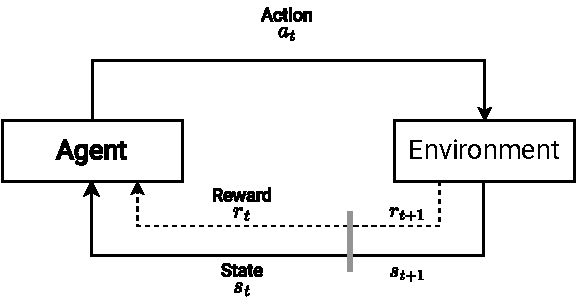
\includegraphics[width=\textwidth]{chapters/img/single-agent-rl.drawio.pdf}
  \caption{Overview of the \ac{rl} framework.}\label{fig:rl:overview}
\end{figure}
\Acl{rl}~\cite{sutton2018reinforcement-learning} serves as a universal framework that h
 as been inspired by the cognitive processes underlying human learning. 
 This paradigm has proven to be highly effective for addressing \emph{control problems}, 
 which are essentially tasks that require decision-making to achieve a particular outcome.
%
The core focus of \ac{rl} is on the \emph{sequential} interactions that occur between \emph{agents} 
 and an \emph{environment} (summarized in \Cref{fig:rl:overview}). 
 Agents are defined as entities capable of performing \emph{actions}, 
 while the environment constitutes everything that is external to the agents 
 and beyond their immediate control.

During each discrete time step, 
 denoted as $t$, an agent observes the current state of the environment, 
 $s_t$ (e.g., the robot position according to a GPS sensor). 
This state encapsulates the set of all observable information at that particular moment. 
The agent then proceeds to select an \emph{action} 
 (e.g., the torque to be applied to engines) 
 $a_t$ in accordance with its \emph{policy} $\pi$. 
A policy serves as a probabilistic mapping that guides the agent in choosing actions 
 based on the current state. 
 Policies can be simple lookup tables or complex neural networks.

As a result of taking this action, 
 the environment transitions to a new state $s_{t+1}$ at the next time step $t+1$. 
 Simultaneously, the agent receives a \emph{reward} $r_{t+1}$, 
 which is a quantitative measure of the efficacy of the action taken, 
 given the state of the environment.

The overarching objective of \ac{rl} is to discover an \emph{optimal} policy, 
 denoted as $\pi^*$, that aims to maximize the long-term return, or cumulative reward, $G$. 
 This is generally achieved through a \emph{trial-and-error} learning process, 
 where agents continually adapt their policies based on the rewards received.

This framework has found extensive applications in a diverse array of domains. 
 For example, \ac{rl} has been used to create advanced algorithms for video games~\cite{DBLP:journals/spm/ArulkumaranDBB17}, 
 allowing for AI agents that can outperform human players. 
% 
In robotics~\cite{DBLP:journals/ijrr/KoberBP13}, 
 \ac{rl} algorithms are enabling machines to learn complex tasks autonomously, 
 from simple object manipulation to navigation in unstructured environments. 
 It is also making significant inroads in networking, 
 particularly in routing algorithms where dynamic decision-making is crucial~\cite{DBLP:journals/comsur/LuongHGNWLK19}.

\subsection{Markov Decision Process}
This general framework is supported by \ac{mdp}, 
 a mathematical model that describes the environment evolution in sequential decision problems. 
%
A \ac{mdp} consists of a tuple $<\RS, \RA, \RP, \RR>$ in which:
\begin{itemize}
  \item $\RS$ denotes the set of states;
  \item $\RA$ is the set of actions;
  \item $\RP(s_{t + 1} | s_t, a_t)$ define the probability to reach some state $s_{t + 1}$ starting from $s_t$ and performing $a_t$ (i.e. transition probability function);
  \item $\RR(s_t, a_t, s_{t+1})$ devise a probabilistic reward function.
\end{itemize}
In \ac{mdp}, $\RP$ is \emph{memory-less}, 
 namely the next environment state depends only on the current state---
 that is the \emph{Markov property}.
%%
%Typically, in \ac{rl} problems, agents do not have access to $\RR$ or $\RP$, 
% but they can rely only on the experience $(s_t, a_t, r_t)$ sampled at a time step. 
%%
Another important concept in \ac{mdp} is the return 
 $G$ defined as the discounted sum of reward a possible future trajectory $\tau$ (i.e. a sequence of time steps):
%%
\begin{equation}
G_{t} = r_t + \gamma r_{t + 1} + \gamma^2 r_{t + 2} + \dots + \gamma^T r_{t + T} = \sum_{k = t}^T \gamma^{k-t} r_k
\end{equation}
%%
Where $0 \leq \gamma \leq 1$ is the \emph{discount factor}, 
 that is how much the future reward impacts the long-term return.
%%
Based on the value of $T$, we can distinguish between \emph{episodic} and \emph{continuous} tasks.
 The foster ones are characterized by a finite number of time steps
  (e.g., a match of chess), while the latter ones are infinite 
  (e.g., a robot that should wander in an unknown environment).
%%
\subsubsection*{Reinforcement Learning Goal}
The \ac{rl} goal can be expressed as the maximization of the \emph{expected} 
 long-term return following a policy $\pi$:
%%
\begin{equation}
J = \mathbb{E_\pi}\Big[ G_t \Big] = \RE_\pi \Big[ \sum_{k = t}^T \gamma^{t-k} r_k \Big] 
\end{equation}
%%
Particularly, in \ac{RL} we want to find the optimal policy $\pi^*$ that maximizes $J$:
%%
\begin{equation}
\pi^* = \arg \max_{\pi} J
\end{equation}
The equation essentially captures the trade-off between immediate and future rewards. 
 The agent aims to select actions based on the policy \(\pi\) 
 that will maximize this expected long-term return. 
 The discount factor \(\gamma\) allows us to model the agent's consideration 
 for future rewards and is a hyperparameter that can be tuned based on the specific problem being solved.

\subsection{Find a policy given a MDP}

$V^\pi$ is the value function that evaluates how good (or bad) a \emph{state} 
 is according to the long-term return following the policy $\pi$ (\emph{expected value}).
% 
It is defined as:
%%
\begin{equation}
V(s)^\pi = \RE_\pi \Big[ G_t | s_t = s \Big]
\end{equation}
%%
$Q^\pi$ is the corresponding value function that evaluates \emph{state-action} pairs:
%%
\begin{equation}
Q(s, a)^\pi = \RE_\pi \Big[ G_t | s_t = s, a_t = a \Big]
\end{equation}
Policies could be defined through value functions. 
 In particular, a greedy policy based on $Q$ function is the one that always chooses 
 the action with the highest value in a certain state:
\begin{equation}
\pi(s) = \arg \max_{a}(Q(s, a))
\end{equation}
\subsubsection{Dynamic programming}
\begin{figure}
  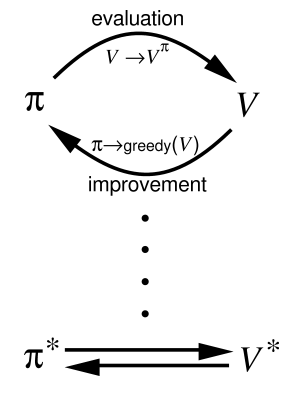
\includegraphics[width=0.3\textwidth]{chapters/img/generalized-policy-improvement.png}
  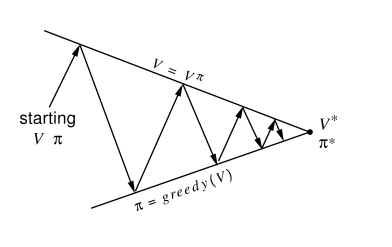
\includegraphics[width=0.65\textwidth]{chapters/img/value-iteration.png}
  \caption{General schema of policy iteration (left) and value iteration (right).}\label{fig:rl:dp}
\end{figure}
Dynamic programming is a family of algorithms that can be used to compute optimal policies 
 given a model of the environment as a \ac{mdp}.
%
In particular, the \emph{Bellman equation} is a fundamental concept in dynamic programming. 
 It is a recursive equation that decomposes the value function into two parts: 
 the immediate reward obtained from the current state and the discounted value of the future state. 
 The Bellman equation for the value function is defined as:
\begin{equation}
V(s) = \sum_{a \in \RA} \pi(a|s) \sum_{s' \in \RS} \RP(s'|s, a) \Big[ \RR(s, a, s') + \gamma V(s') \Big]
\end{equation}
%
Similarly, the Bellman equation for the $Q$ function is defined as:
\begin{equation}
Q(s, a) = \sum_{s' \in \RS} \RP(s'|s, a) \Big[ \RR(s, a, s') + \gamma \sum_{a' \in \RA} \pi(a'|s') Q(s', a') \Big]
\end{equation}
%
The Bellman equation is the basis for many algorithms that solve \ac{mdp},
two most notable are \emph{value iteration} and \emph{policy iteration} (\Cref{fig:rl:dp}).
\subsection{Value iteration}
Value iteration is an iterative algorithm used to compute the optimal value function \(V^*\) and, consequently, the optimal policy \(\pi^*\). 
 The algorithm is particularly useful when the state and action spaces are too large to solve directly through analytical methods. 
 It is based on the principle of optimality, which states that if an optimal policy \(\pi^*\) exists, then it must satisfy the Bellman optimality equation.

The algorithm starts by initializing \(V(s)\) for all states \(s\) to some arbitrary values, often zeros. 
 It then iteratively updates the value of each state \(s\) using the Bellman optimality equation until the value function converges to \(V^*\). 
 The convergence is usually checked by measuring the difference between successive value functions and comparing it against a small threshold \(\epsilon\):
\begin{equation}
V_{k+1}(s) = \max_{a \in \mathcal{A}} \sum_{s' \in \mathcal{S}} \RP(s'|s, a) \Big[ \RR(s, a, s') + \gamma V_k(s') \Big]
\end{equation}

The \(\max\) operation ensures that the value function is updated to reflect the best possible action at each state. 
 The term \(\gamma V_k(s')\) represents the discounted future rewards, and \(R(s, a, s')\) is the immediate reward. 
 The transition probability \(P(s'|s, a)\) models the uncertainty in the environment.

After the value function has converged to \(V^*\), the optimal policy \(\pi^*\) can be extracted. The policy is determined by selecting the action that maximizes the expected return in each state, as given by:

\begin{equation}
\pi^*(s) = \arg \max_{a} \sum_{s' \in \mathcal{S}} P(s'|s, a) \Big[ R(s, a, s') + \gamma V^*(s') \Big]
\end{equation}
This policy is guaranteed to be optimal with respect to the original MDP.


\subsection{Policy Iteration}
Policy iteration is another dynamic programming algorithm used for finding the optimal policy \(\pi^*\). 
 Unlike value iteration, policy iteration consists of two main steps: 
 \emph{policy evaluation} and \emph{policy improvement}, 
 which are repeated iteratively until the policy converges to \(\pi^*\):
\begin{itemize}
  \item policy evaluation: in this step, the value function \(V^\pi\) for the current policy \(\pi\) is computed until it stabilizes. The update rule is:

  \begin{equation}
  V_{k+1}(s) = \sum_{a \in \mathcal{A}} \pi(a|s) \sum_{s' \in \mathcal{S}} P(s'|s, a) \Big[ R(s, a, s') + \gamma V_k(s') \Big]
  \end{equation}
  \item policy improvement: after evaluating \(V^\pi\), the policy is updated to be greedy with respect to \(V^\pi\):
  \begin{equation}
  \pi'(s) = \arg \max_{a} \sum_{s' \in \mathcal{S}} P(s'|s, a) \Big[ R(s, a, s') + \gamma V^\pi(s') \Big]
  \end{equation}
\end{itemize}
The algorithm then returns to the policy evaluation step, using the new policy \(\pi'\), and continues until the policy no longer changes.
 
%The objective in value-based methods is to find the best value function (whether $Q$ or $V$), defined as:
%\begin{iequation}
%Q^* = \arg \max_{\pi}(Q^\pi(s, a)) \; \text{or} \; V^* = \arg \max_{\pi}(V^\pi(s))
%\end{iequation}
%Consequently, when we have found $Q^*$, an optimal policy is straightforwardly defined:
%\begin{equation}
%\pi^*(s) = \underset{a}{\text{argmax}}(Q^*(s, a))
%\end{equation}
\subsection{Find a policy without an MDP}
While dynamic programming methods like value iteration and policy iteration offer powerful ways to find the optimal policy \(\pi^*\), 
 they come with a significant limitation: 
 the need for a complete model of the environment. 
 Specifically, these algorithms require knowledge of the transition probability function \(\RP\) and the reward function \(\RR\). 
 In many real-world applications, these functions are either unknown or too complex to model accurately. 
 This is where \emph{model-free} algorithms come into play.
 In the following sections, we will discuss two such algorithms' family: 
 Monte Carlo methods and Temporal Difference methods.
\subsubsection{Monte Carlo methods}
Monte Carlo methods offer a way to find an optimal policy \(\pi^*\) without requiring a model of the environment. 
 These methods rely on sampling sequences of states, actions, and rewards from actual or simulated interactions with the environment. 
 By averaging these samples, the agent can estimate the value functions \(V(s)\) and \(Q(s, a)\), which can then be used to improve the policy.

The core idea is to run multiple episodes, 
 from start to finish, and then update the value estimates based on the returns observed. 
 The value of a state \(s\) or a state-action pair \((s, a)\) is estimated as the average of the returns that have followed that state or state-action pair across multiple episodes.

\begin{equation}
V(s) = \frac{1}{N} \sum_{i=1}^{N} G_t^{(i)}
\end{equation}

\begin{equation}
Q(s, a) = \frac{1}{N} \sum_{i=1}^{N} G_t^{(i)}
\end{equation}

Where \(N\) is the number of times the state or state-action pair has been visited, and \(G_t^{(i)}\) is the return following the \(i\)-th visit.

Once the value functions are estimated, 
 the policy can be improved by making it greedy with respect to these estimated values. 
%
In this context, the \emph{exploration-exploitation} trade-off is crucial.
%
In fact, the agent should explore the environment to discover new states and actions that could lead to higher rewards,
  but it should also exploit the knowledge it has already acquired to maximize the expected return.
%
Monte Carlo methods are particularly useful when the state and action spaces are large, making it impractical to enumerate all possible state-action pairs. However, they do require the episodes to be finite and can be computationally expensive due to the need for multiple samples to obtain accurate estimates.

\paragraph*{Exploration-Exploration dilemma}
In these algorithms, the agent should explore the environment to discover new states and actions that could lead to higher rewards,
  but it should also exploit the knowledge it has already acquired to maximize the expected return.
  This is the so-called \emph{exploration-exploitation} trade-off.
  This is not only a matter in Monte Carlo methods, but it is a general problem in model-free algorithms, in which agent should learn a policy without a model of the environment.
%
There are several ways to address this dilemma, 
 but the most common approach is to use an \emph{$\epsilon$-greedy} policy. 
 This policy selects a random action with probability \(\epsilon\) and the greedy action with probability \(1 - \epsilon\). 
 The value of \(\epsilon\) is typically set to a small value, 
 such as 0.1 or 0.2, 
 to ensure that the agent explores the environment sufficiently.
%

\subsubsection{Temporal difference methods}
Temporal difference methods are a class of \emph{model-free} and \emph{value-based} algorithms 
 that allow the agent to learn optimal behaviour directly from its interactions with the environment, without requiring a model. 
 TD methods combine ideas from both Monte Carlo methods and dynamic programming to provide a flexible and powerful approach to reinforcement learning.

One of the simplest TD methods is \emph{TD-Learning}~\cite{DBLP:journals/ml/Sutton88}, 
 which updates the value function \(V(s)\) based on the temporal difference error \(\delta\), 
 defined as \( \delta = R(s, a, s') + \gamma V(s') - V(s) \). 
 The value function is then updated using \( V(s) \leftarrow V(s) + \alpha \delta \), where \(\alpha\) is the learning rate.

Starting from this intuition two main approaches have been developed: 
 \emph{Q-learning}~\cite{DBLP:journals/ml/WatkinsD92} and \emph{SARSA}~\cite{10.5555/3312046}. 

 \paragraph*{Q-Learning}

 Q-Learning is an off-policy TD algorithm that focuses on learning the action-value function \(Q(s, a)\). The update rule for Q-Learning is:
 \begin{equation}
 Q(s, a) \leftarrow Q(s, a) + \alpha \Big[ R(s, a, s') + \gamma \max_{a'} Q(s', a') - Q(s, a) \Big]
 \end{equation}
 The algorithm is termed ``off-policy'' because it learns the value of the optimal policy regardless of the policy being followed, 
  thanks to the \(\max_{a'}\) term in the update rule.
 
 \paragraph*{SARSA}
 SARSA (State-Action-Reward-State-Action) is an on-policy TD algorithm. 
  Unlike Q-Learning, SARSA takes into account the current policy \(\pi\) during the learning process. The update rule for SARSA is:
 \begin{equation}
 Q(s, a) \leftarrow Q(s, a) + \alpha \Big[ R(s, a, s') + \gamma Q(s', a') - Q(s, a) \Big]
 \end{equation}
 where \(a'\) is the action taken under the current policy \(\pi\).
 
 Both Q-Learning and SARSA have their own advantages and disadvantages. 
  Q-Learning tends to find the optimal policy faster but may be more sensitive to noise. SARSA, being an on-policy method, is more conservative and tends to find safer policies, especially when the policy involves some level of risk or uncertainty.

\subsection{Policy Gradient Methods}

While temporal difference methods and monte carlo methods focus on learning value functions to derive optimal policies, \emph{policy gradient} methods take a different approach. 
  They aim to directly optimize the policy \(\pi\) itself, 
  rather than first estimating value functions. 
  This is particularly useful in environments with high-dimensional action spaces or continuous action spaces, where value-based methods may struggle.
  Moreover, in this way, it is possible to learn stochastic policies,
    which are often more robust and flexible than deterministic policies.

Policy gradient methods optimize the policy by ascending the gradient of the expected return with respect to the policy parameters \(\theta\). 
Mathematically, this can be expressed as:
\begin{equation}
\theta \leftarrow \theta + \alpha \nabla_\theta J(\theta)
\end{equation}
where \(J(\theta)\) is the expected return when following policy \(\pi_\theta\), and \(\alpha\) is the learning rate.

One of the foundational algorithms in this category is the REINFORCE algorithm~\cite{DBLP:conf/nips/SuttonMSM99}: it is one of the earliest and most straightforward policy gradient methods. 
It estimates the gradient of the expected return by sampling trajectories from the current policy \(\pi_\theta\). 
After each episode, the algorithm adjusts the policy parameters \(\theta\) in the direction that increases the expected return.
%
The core equation for the REINFORCE algorithm is:
\begin{equation}
\nabla_\theta J(\theta) = \mathbb{E}_{\tau \sim \pi_\theta} \left[ \sum_{t=0}^{\infty} \nabla_\theta \log \pi_\theta(a_t | s_t) G_t \right]
\end{equation}

Here, \(\tau\) represents a trajectory sampled from the policy \(\pi_\theta\), and \(G_t\) is the return from time \(t\). 
 The term \(\nabla_\theta \log \pi_\theta(a_t | s_t)\) is the log-likelihood gradient, 
 and \(G_t\) serves as a sample estimate for how good the action \(a_t\) is in state \(s_t\).

The REINFORCE algorithm operates in an episodic setting, 
 meaning it waits until the end of each episode to update the policy. 
 This makes it well-suited for tasks where the episode termination is natural, such as games or tasks with a fixed time horizon. 
 However, one drawback of REINFORCE is that it can have high variance in its updates, which can make the training process unstable. 
 Various techniques, such as using a \emph{baseline} or employing advanced variance reduction methods, have been developed to mitigate this issue.

REINFORCE is particularly useful when the action space is high-dimensional or continuous, where traditional value-based methods like Q-Learning may struggle. 


\section{Multi-agent}
\begin{figure}
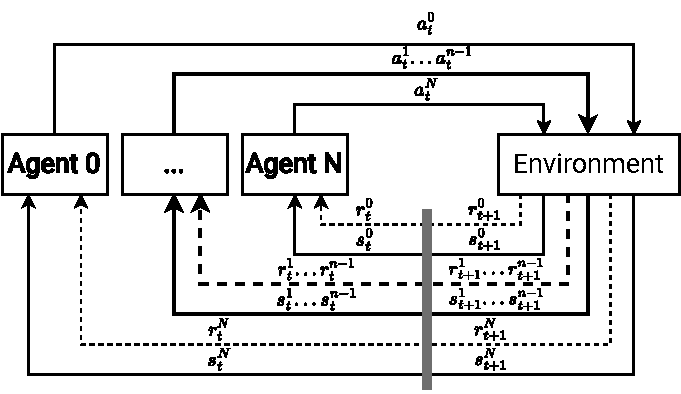
\includegraphics[width=\textwidth]{chapters/img/multi-agent-rl.drawio.pdf}
\caption{Overview of the \ac{marl} framework.}\label{fig:marl:overview}
\end{figure}
In the evolving landscape of \ac{rl}, the concept of \ac{marl} stands as a natural extension of the foundational \ac{rl} principles. 
 While traditional \ac{rl} generally focuses on the interactions between a single agent and an environment, 
 \ac{marl} broadens the scope to include multiple agents, 
 each with their own objectives, policies, and decision-making processes.

The basic setting in \ac{marl} comprises multiple agents interacting either \emph{cooperatively}, \emph{competitively}, or in a \emph{mixed} fashion within a shared environment---more details in the following sections. 
 Each agent $i$ continues to observe its own state $s_{t}^{i}$, select actions $a_{t}^{i}$ according to its policy $\pi^{i}$, and receive rewards $r_{t+1}^{i}$.
 However, in \ac{marl}, 
 an agent's actions can directly or indirectly influence the states and rewards of other agents, 
 thereby increasing the complexity of the learning problem.
The key challenge in \ac{marl} is to develop robust algorithms that enable agents to learn optimal policies in these complex, often non-stationary, environments. Classic \ac{rl} algorithms often require modifications to accommodate the multi-agent setting. For instance, the concept of a joint action space, a state space extended to multiple agents, and a composite reward function are essential considerations.
\subsection{Markov Games}
The formalization of multi-agent reinforcement learning (MARL) typically extends the standard Markov Decision Process (MDP) framework to account for multiple agent. One of the most straightforward extensions is the Markov Game. 
 In this formalization, each agent has its own state, action, and reward function, and the joint actions of all agents determine the transition dynamics and rewards: 
\begin{equation}
Markov\_Game = \langle \mathcal{N}, \mathcal{S}, \mathcal{A}_1, \ldots, \mathcal{A}_N, \mathcal{P}, \mathcal{R}_1, \ldots, \mathcal{R}_N \rangle
\end{equation}
Where:
\begin{itemize}
    \item $\mathcal{N}$ is the number of agents.
    \item $\mathcal{S}$ is the joint state space.
    \item $\mathcal{A}_i$ is the action space of agent $i$.
    \item $\mathcal{P}$ is the joint transition probability function.
    \item $\mathcal{R}_i$ is the reward function for agent $i$.
\end{itemize}

\subsection{Taxonomies}
Multi-agent systems can be categorized based on various criteria:

\begin{itemize}
    \item \textbf{Communication}: Agents can either communicate directly with each other or have no communication.
    \item \textbf{Cooperation Level}: Systems can be fully cooperative, fully competitive, or mixed (both cooperative and competitive).
    \item \textbf{Adversarial Nature}: Some systems have agents with opposing goals, making them adversarial.
\end{itemize}

\subsection{State-of-the-art}
Recent advancements in MARL have led to the development of algorithms that can handle complex interactions between agents. Some state-of-the-art algorithms include Proximal Policy Optimization (PPO) for multi-agent settings, MADDPG (Multi-Agent Deep Deterministic Policy Gradient), and QMIX.

\section{Many-agent}
The \ac{marl} framework, even if consider multiple agents,
  still assumes that the number of agents is small (i.e. $N \leq 2$).
  For that reason, solutions that work well in \ac{marl} settings may not be suitable for \emph{many-agent} scenarios.

In this thesis, we consider \emph{homogeneous \ac{MAARL}}~\cite{yang2021many}, 
 where the set of agents is large ($N \gg 2$) and each agent is \emph{interchangeable} and \emph{indistinguishable}.
%
This research area is relevant in the context of large-scale systems 
 where collective intelligence emerges from local and repeated interaction of simple entities, like in \ac{cpsw}.
%
In such many-agent scenarios, 
 the implementation of fully decentralized learning is often unfeasible due to the large number of learning agents, 
 which makes the system non-stationary and difficult to manage. 
%
Conversely, a centralized controller capable of coordinating 
 the entire system may not be a viable solution due to scalability concerns. 
 To address this challenge, a practical solution is the adoption of \emph{\ac{CTDE}} approach.
%
The idea is to learn a policy at simulation time when there is a collective view of the system, 
 and then at runtime use that policy but only with local observations. 
%This approach creates policies that are influenced by global information but only require local information to function at runtime. 
%
The typical approach in such cases is based on actor-critic systems~\cite{DBLP:conf/nips/LoweWTHAM17,wu2022more,song2022ctds,song2022centralized},
  where the \emph{actor} is the distributed policy (with only local information) and the critic is a neural network that takes the overall system state.
%
%In fact, the first works in this direction were discussed precisely swarm robotics, %\lukas{what does this mean `in the last field'?}
% exploring new models (e.g., swarMDP~\cite{DBLP:conf/atal/SosicKZK17}) and learning algorithms capable of extrapolating a policy representing the entire system.  \lukas{This sentence still needs rework.}
%Modern approaches, however, 
% have started to consider the use of 
% Recently, deep learning approaches have been considered 
% to synthesise robust controllers capable of generalizing to new tasks. 
%In this context, mean-field reinforcement learning~\cite{pmlr-v80-yang18d} is certainly noteworthy. 
Mean-field RL~\cite{pmlr-v80-yang18d} is one of such concrete applications of \ac{CTDE} 
 where the interactions among the population of agents are estimated by considering either the effect of a single agent and the average impact of the entire population or the influence of neighbouring agents.
%
Some known approaches using mean-field reinforcement learning include Q-mean, 
 which is an extension of Q-learning to mean-field settings~\cite{yang2018mean}, 
 and actor-critic mean-field~\cite{frikha2023actor}, which combines actor-critic algorithms with mean-field approximations. 
%
These approaches have shown promising results in various domains, such as multi-agent coordination 
 and decentralized control, and are actively being researched and developed for further applications.

\subsection{Formalization}
\subsubsection{SwarMDP}
A SwarMDP is characterized by a \emph{swarming agent} ($\mathbb{A}$) and the dynamics of the environment ($\mathbb{E}$).
Specifically, $\mathbb{A}$ is a tuple ($\mathcal{S}, \mathcal{O}, \mathcal{A}, \mathcal{R}, \pi$) where:
\begin{itemize}
  \item $\mathcal{S, O, A}$ are the set of local states, observations (or features), and actions, respectively;
  \item $\mathcal{R}: \mathcal{S} \rightarrow \mathbb{R}$ is the reward function, which is influenced by the environment;
  \item $\pi: \mathcal{O} \rightarrow \mathcal{A}$ is the policy function, which maps the observations to the actions: it could be deterministic or stochastic.
\end{itemize}
Starting from this definition, the environment $\mathbb{E}$ is defined as a tuple ($\mathcal{P}, \mathbb{A}, \mathcal{T}, \xi$), where:
\begin{itemize}
  \item $\mathcal{P}$ is the total number of agents in the systems (the agent population), which is assumed to be fixed;
  \item $\mathbb{A}$ is the defined agent prototype that rules each agent $v \in P$;
  \item $\mathcal{T}: \mathcal{S}^P \times \mathcal{A}^P \times \mathcal{S}^P \rightarrow \mathbb{R}$ is the transition  global function, which is influenced by the actions of the agents and returns a collective reward -- this is typically not known by the swarming agents;
  \item $\xi: \mathcal{S^P} \rightarrow \mathcal{O^P}$ is the global observation model of the systems.
\end{itemize}
\subsubsection{Networked Markov Decision Process}

\subsection{State-of-the-art}
In many-agent systems, the sheer number of agents makes traditional MARL techniques computationally infeasible. Recent advancements focus on scalable algorithms and techniques like mean-field theory to approximate the interactions between agents. Some notable algorithms include Mean Field Q-learning and Graph Neural Networks for many-agent systems.

\section{Gran-challenges}
